\documentclass[]{standalone}

\usepackage{adjustbox}

\usepackage{amsmath}

\usepackage{mathrsfs}

\usepackage{tikz}
\usetikzlibrary{arrows, patterns, decorations.pathmorphing, backgrounds, positioning, fit, petri, shapes, trees, matrix, chains, decorations, decorations.pathreplacing, decorations.fractals, calc,snakes,trees, decorations.markings}

\usepackage{color}
\definecolor{soton}{RGB}{7,51,71}
\colorlet{comms}{red!50!yellow}
\colorlet{payld}{pink!50!purple}
\colorlet{obdh}{green!50!black}

\begin{document}

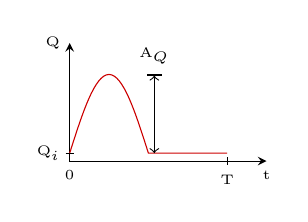
\begin{tikzpicture}

\draw[stealth-stealth] (0,1.5) node[left] {\tiny{Q}} -- (0,0) node[below] {\tiny{0}} --  (2.5,0) node[below] {\tiny{t}};
\draw[red!80!black] (0,0.1) node[left, black] {\tiny{Q$_i$}} sin (0.5,1.1) cos (1,0.1) -- (2,0.1);
\draw (-0.05,0.1) -- (0.05,0.1);
\draw[<->|] (1.075,0.1) -- (1.075,1.1) node[above] {\tiny{A$_Q$}};
\draw (2,-0.05) node[below] {\tiny{T}} -- (2,0.05);


\end{tikzpicture}


\end{document}